\documentclass{article}

% if you need to pass options to natbib, use, e.g.:
%     \PassOptionsToPackage{numbers, compress}{natbib}
% before loading neurips_2018

% ready for submission
% \usepackage{neurips_2018}

% to compile a preprint version, e.g., for submission to arXiv, add add the
% [preprint] option:
%     \usepackage[preprint]{neurips_2018}

% to compile a camera-ready version, add the [final] option, e.g.:
     \usepackage[final]{nips_2018}

% to avoid loading the natbib package, add option nonatbib:
%     \usepackage[nonatbib]{neurips_2018}

\usepackage[utf8]{inputenc} % allow utf-8 input
\usepackage[T1]{fontenc}    % use 8-bit T1 fonts
\usepackage{hyperref}       % hyperlinks
\usepackage{url}            % simple URL typesetting
\usepackage{booktabs}       % professional-quality tables
\usepackage{amsfonts}       % blackboard math symbols
\usepackage{nicefrac}       % compact symbols for 1/2, etc.
\usepackage{microtype}      % microtypography
\usepackage{graphicx}
\usepackage{CJKutf8}


\title{《人工神经网络》大作业中期报告}

% The \author macro works with any number of authors. There are two commands
% used to separate the names and addresses of multiple authors: \And and \AND.
%
% Using \And between authors leaves it to LaTeX to determine where to break the
% lines. Using \AND forces a line break at that point. So, if LaTeX puts 3 of 4
% authors names on the first line, and the last on the second line, try using
% \AND instead of \And before the third author name.

\author{%
  陶天骅 \\
  2017010255 \\
  计算机系 \\
  \texttt{tth17@mails.tsinghua.edu.cn} \\
  %% examples of more authors
  \And
  杨雅儒\\
  2017011071 \\
  计算机系 \\
  \texttt{yangyr17@mails.tinghua.edu.cn
  } \\
  %% \And
  %% Coauthor \\
  %% Affiliation \\
  %% Address \\
  %% \texttt{email} \\
}

\begin{document}
% \nipsfinalcopy is no longer used
\begin{CJK*}{UTF8}{gbsn}
\maketitle


\section{引言}

本课题希望构建一个神经网络以及一些简单的界面,可以根据用户提供的一些特征的比例,自动生成一张风景图片。程序界面示意图如下。

\section{问题陈述}

我们希望基于AutoEncoder和GAN模型,构建能自动生成风景画的网络。

\section{初步实验结果}

收集的数据集包括了5700多张风景图片。通过缩放处理后可以作为300 x 300或者128 x 128的图片集。一些示例图片如下所示。

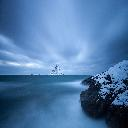
\includegraphics{./data1.jpg}
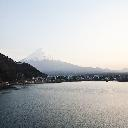
\includegraphics{./data2.jpg}
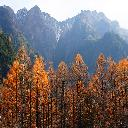
\includegraphics{./data3.jpg}

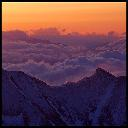
\includegraphics{./data7.jpg}
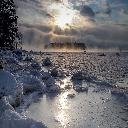
\includegraphics{./data8.jpg}
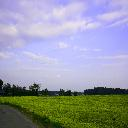
\includegraphics{./data9.jpg}


目前已构造一个AutoEncoder网络和DCGAN网络。

AutoEncoder可以将一个较小的图片进行编码压缩后,再重新解码,尝试重构该图片。

输入与输出图片如下所示。

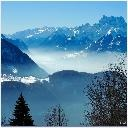
\includegraphics{./target.jpg}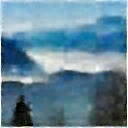
\includegraphics{./gen.jpg}

我们希望继续拓展AutoEncoder模型,使其能对图中的特征分类。

DCGAN是使用了卷积层的GAN,通过在收集的数据集上进行训练,GAN模型获取了一些风景图的基本风格特征,但是很模糊,没有学习到细致的特征。训练中生成的一些图(训练半小时后)如下所示。

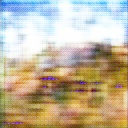
\includegraphics{./eg1.jpg}
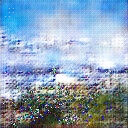
\includegraphics{./eg2.jpg}
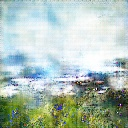
\includegraphics{./eg4.jpg}
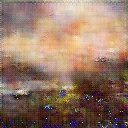
\includegraphics{./eg5.jpg}



\section{目前的困难}

生成高分别率的图片有困难。困难一方面在于训练高分辨率时,原来的模型会失效,图片扭曲严重;另一方面训练时间更长,计算资源不足。

GAN生成图片时加入特征的选择。这需要结合AutoEncoder和GAN两种网络,正在探索融合的方法。


\section{未来计划}

引入 Fréchet Inception Distance (FID) 判别指标[1]来量化GAN生成的图片的逼真程度。

探索在GAN加入基于Style和Attention的机制的方法。

构造更加复杂的网络结构。

尝试将数据集进行手动分类,如分为山、森林、海等类别。考虑增加标签后进行训练。

\section*{参考文献}

\small

[1] Karras, T., Laine, S., Aila, T. (2018). A Style-Based Generator Architecture for Generative Adversarial Networks. 

[2] M. Heusel, H. Ramsauer, T. Unterthiner, B. Nessler, and S. Hochreiter. GANs trained by a two time-scale update rule converge to a local Nash equilibrium. In Proc. NIPS, pages 6626–6637, 2017.


\end{CJK*}
\end{document}


